\chapter{Progettazione} %------------------------------ CHAPTER TITLE
\thispagestyle{empty}

\newpage
\section{Architettura}
L'architettura ad alto livello che si vuole utilizzare è molto semplice. Essa prevede l'implementazione di un componente SAPI~5 e lo sviluppo di un canale di comunicazione con un engine TTS.
Per facilitare lo svolgimento del progetto si è scelto di utilizzare, in congiunta con il committente, un esempio guida chiamato SALB.
Il progetto SALB implementa l'interfaccia SAPI~5 e al suo interno esegue delle chiamate ad un engine TTS.
Partendo da questo esempio andranno sostituite le varie parti che dovranno subire delle modifiche per poi proseguire fino ad ottenere il prodotto desiderato.
Riassumendo, i vari componenti che verranno utilizzati sono:
\begin{description}
	\item[Interfaccia SAPI~5] interfaccia messa a disposizione dal sistema operativo Microsoft Windows che permette di implementare le funzionalità di sintesi e riconoscimento vocale;
	\item[Implementazione interfaccia SAPI~5] seguendo la specifica SAPI~5 si andranno ad implementare le varie funzionalità di sintesi vocale che potranno essere messe a disposizione attraverso l'interfaccia. L'implementazione fornita dipenderà da un engine TTS.
	\item[Engine TTS] engine di sintesi vocale messo a disposizione dall'azienda. Gli engine di sintesi vocale saranno MaryTTS e Speect.
\end{description}
\newpage

\section{Descrizione dei componenti}
	\subsection{Interfaccia SAPI~5}
	  \begin{figure}[H]
	  	\centering
	  	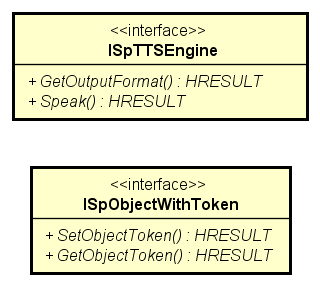
\includegraphics{images/sapi5-interface.png}
	  	\caption{Interfaccia SAPI~5}
	  \end{figure}
 
L'interfaccia SAPI~5 è stata progettata per facilitare il lavoro agli sviluppatori di applicazioni e di engine TTS. Il suo scopo è quello di standardizzare il modo con cui avviene la comunicazione tra applicazioni ed engine TTS. Uno dei task che viene semplificato, utilizzando questa interfaccia, è la gestione del flusso audio. Questo permette agli sviluppatori focalizzarsi maggiormente nello sviluppo dell'engine e non di come il suo output audio venga gestito.
Le interfacce che verranno utilizzate sono ISpTTSEngine e ISpObjectWithToken.
     \subsubsection{ISpObjectWithToken}
     L'interfaccia ISpObjectWithToken permette di creare e reperire le informazioni associate ad un oggetto. Nella maggior parte dei casi l'oggetto viene associato ad una voce.\\
     \textbf{Metodi}
     \begin{itemize}
     	\item \texttt{SetObjectToken(): HRESULT} imposta le proprietà dell'oggetto passato come parametro.\\
     	\textbf{Argomenti}
		\begin{itemize}
			\item \texttt{pToken: ISpObjectToken} puntatore all'oggetto che deve essere impostato.
		\end{itemize}
     	\textbf{Valori di ritorno}
		\begin{itemize}
		 	\item \texttt{S\_OK} se la funzione non ha generato errori;
		 	\item \texttt{E\_POINTER} se il parametro \texttt{pToken} non è valido o è malformato;
		 	\item \texttt{E\_OUTOFMEMORY} se la memoria disponibile non è sufficiente;
		 	\item \texttt{FAILED(hr)} se c'è un errore da ritornare. 
		 \end{itemize}
	    
	     \item \texttt{GetObjectToken(): HRESULT} serve per ottenere un oggetto settato in precedenza. L'oggetto verrà restituito come parametro.\\
	     \textbf{Argomenti}
		 \begin{itemize}
		     \item \texttt{ppToken: ISpObjectToken} indirizzo dell'oggetto richiesto.
		 \end{itemize}
	     \textbf{Valori di ritorno}
		 \begin{itemize}
		    \item \texttt{S\_OK} se la funzione non ha generato errori;
		    \item \texttt{E\_POINTER} se il parametro \texttt{ppToken} non è valido o è malformato;
		    \item \texttt{E\_OUTOFMEMORY} se la memoria disponibile non è sufficiente;
	     	\item \texttt{FAILED(hr)} se c'è un errore da ritornare. 
	     \end{itemize}
     \end{itemize}
      
     \subsubsection{ISpTTSEngine}
     L'interfaccia ISpTTSEngine 
     \textbf{Metodi}
   
 